\documentclass[../main.tex]{subfiles}

\begin{document}
	\section{Composites}
	Les fibres de verre et de carbones sont des exemples de composites, les fibres de carbonnes font environ $10\mu$ de large. Ils sont maintenant utilisé sur des fuselages d'avions. Les fibres sont la plupart du temps mélangé avec des polymères. Ils sont anisotropes, c'est à dire que leurs propriétés changent par rapport à l'orientation des fibres.
	\section{Propriété}
	\begin{figure}
		\begin{center}
			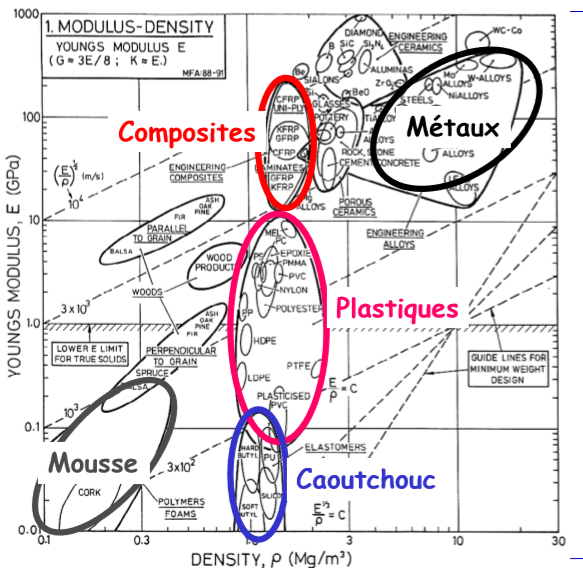
\includegraphics[width=10cm]{CompositeModulus.png}
			\caption{\label{compositemodulus}Les composites ont une rigidité proches des métaux tout en gardant une densité proche de 1}
		\end{center}
	\end{figure}
	Les composites ont une rigidité proche des métaux, malgré ceci, ils peuvent flotter sur l'eau avec des densités plus faibles \ref{compositemodulus}. On peut travailler différemment les composites, soit en unidirectionnels, qui sont très adapté dans les situations qui recquierent des efforts directionnel, alors qu'on peut les tisser pour par exemple avec des gilet kevlar.
	\subsection{Polymères et composites organiques}
	On utilise en particulier, les phénoliques car ils résistent au feu. C'est utilisé en électronique en majorité. 
	\section{Composition}
	On a différents types de combinaison. Un matériau est constitué d'une matrice continue contenant un rendort sous forme de fibres ou de particules. 
	\subsection{Matrice avec particules}
	\begin{figure}
		\begin{center}
			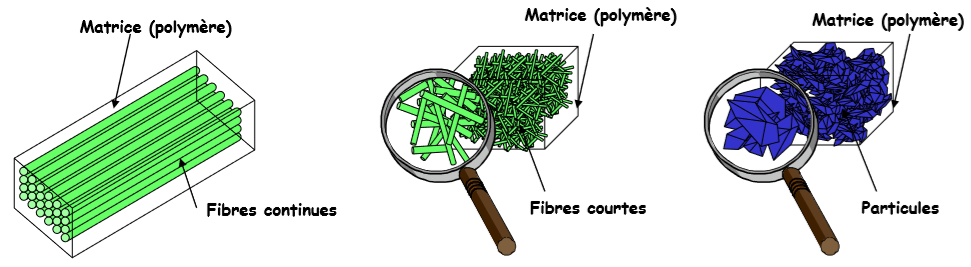
\includegraphics[width=19cm]{CompositeMat.png}
			\caption{\label{compositemat}De gauche a droite, matrice + fibres continues, matrice + fibre courte, matrice + particules}
		\end{center}
	\end{figure}
	%TODO
	

\end{document}